\documentclass[10pt, a4paper, twocolumn]{article}

% Core packages
\usepackage{amsmath, amssymb, amsthm}
\usepackage{mathpazo} % Palatino font for text and math
\usepackage{sourcesanspro} % Sans serif font for headers
\usepackage{graphicx}
\usepackage{booktabs}
\usepackage{hyperref}
\usepackage{geometry}
% \usepackage[utf8]{inputenc} % Not needed for XeLaTeX
\usepackage{float}
\usepackage{xcolor}
\usepackage{tcolorbox}
\usepackage{listings}
\usepackage{sectsty} % For custom section headers

% Style section headers
\allsectionsfont{\sffamily\bfseries\color{darkgray}}

\definecolor{codegreen}{rgb}{0,0.6,0}
\definecolor{codegray}{rgb}{0.5,0.5,0.5}
\definecolor{codepurple}{rgb}{0.58,0,0.82}
\definecolor{backcolour}{rgb}{0.95,0.95,0.92}
\definecolor{sidebarcol}{RGB}{240, 240, 245}
\definecolor{sidebarline}{RGB}{100, 100, 120}

\lstdefinestyle{mystyle}{
    backgroundcolor=\color{backcolour},
    commentstyle=\color{codegreen},
    keywordstyle=\color{magenta},
    numberstyle=\tiny\color{codegray},
    stringstyle=\color{codepurple},
    basicstyle=\ttfamily\footnotesize,
    breakatwhitespace=false,
    breaklines=true,
    captionpos=b,
    keepspaces=true,
    numbers=left,
    numbersep=5pt,
    showspaces=false,
    showstringspaces=false,
    showtabs=false,
    tabsize=2
}
\lstset{style=mystyle}

% Page layout
\geometry{margin=2.5cm}

% Theorem environments for the guide
\newtheorem{definition}{Definition}
\newtheorem{theorem}{Theorem}
\newtheorem{example}{Example}

% Custom boxes for "Key Intuition"
\newtcolorbox{intuition}{
    colback=blue!5!white,
    colframe=blue!75!black,
    title=Key Intuition
}

% Custom sidebar box (now generalized)
\tcbset{
    emicstyle/.style={
        colback=sidebarcol,
        colframe=sidebarline,
        fonttitle=\sffamily\bfseries,
        arc=0mm,
        boxrule=0.5pt,
        leftrule=4pt
    }
}

\newtcolorbox{sidebar}[1]{
    emicstyle,
    title=#1
}

% Floating Figure Box
\newtcolorbox[blend into=figures]{emicfigure}[2][]{
    emicstyle,
    float,
    title={#2},
    colback=white,
    #1
}

% Floating Table Box
\newtcolorbox[blend into=tables]{emictable}[2][]{
    emicstyle,
    float,
    title={#2},
    colback=white,
    #1
}

% Floating Code Box
% We track a custom counter for listings to match the look
\newcounter{emiclisting}
\newtcolorbox{emiclisting}[2][]{
    emicstyle,
    float,
    code={\refstepcounter{emiclisting}},
    title={Code Listing \theemiclisting: #2},
    #1
}

% Metadata
\title{\textbf{\sffamily A Guide to Computational Mechanics}}
\author{John S Azariah\\
\small University of Technology, Sydney\\
\small \texttt{john.azariah@student.uts.edu.au}}
\date{\today}

\begin{document}

\maketitle

\begin{abstract}
    How do we find structure in randomness? This guide introduces \textit{Computational Mechanics}, a framework for inferring causal models from time-series data. We build up from basic Information Theory to the construction of $\epsilon$-machines---optimal predictors of the future. We demonstrate these concepts using the "Golden Mean" process and the Logistic Map, verifying theoretical bounds along the way. This document is generated from a reproducible pipeline using the \texttt{emic} Python library.
\end{abstract}

\tableofcontents
\newpage

\section{Introduction}
Imagine you are watching a stream of data go by. It might be the ups and downs of a stock market ticker, the sequence of DNA bases in a genome, or the turbulent velocity of a fluid.

At first glance, it looks random. But is it?

We are often tasked with finding \textit{patterns} in data. But what exactly is a pattern? In statistics, we talk about "correlation". In dynamical systems, we talk about "attractors". Computational Mechanics provides a different answer: a pattern is a structure that allows us to \textbf{predict}.

To understand a process is to be able to predict its future given its past. If a process is perfectly random (like a coin flip), the past tells us nothing about the future. If it is periodic (like a clock), the past tells us everything. Most interesting processes lie somewhere in between: they are \textit{structured stochastic processes}.

\begin{sidebar}{Intrinsic Computation}
Computational Mechanics views nature not just as a system of energy, but as a system of \textit{information processing}. The universe computes. A process ``stores'' information from the past (memory) and ``processes'' it to generate the future. Our goal is to reverse-engineer this computation from the data alone.
\end{sidebar}

This guide will walk you through the framework of Computational Mechanics \cite{shalizi2000computational}. We will not just learn definitions; we will construct the optimal predictive model---the $\epsilon$-machine---from scratch. We will see how to measure the "memory" of a process and verify that our models are as simple as possible, but no simpler.


\section{Preliminaries: The Language of Uncertainty}
\label{sec:preliminaries}
Before we can talk about complexity and structure, we need a language to talk about uncertainty. That language is Information Theory.

\subsection{Entropy: A Measure of Surprise}
The foundational quantity is Shannon Entropy, denoted $H$. It measures the average uncertainty or "surprise" inherent in a random variable.

If we have a random variable $X$ that can take values $x$ from an alphabet $\mathcal{A}$ with probability $P(x)$, the entropy is:
\begin{equation}
    H[X] = - \sum_{x \in \mathcal{A}} P(x) \log_2 P(x)
\end{equation}
We measure entropy in \textbf{bits}.

\begin{sidebar}{Why Bits?}
    Shannon chose base 2 for his logarithms, giving us the \textit{bit} (binary digit). A bit represents a choice between two equally likely alternatives. However, other bases are possible:
    \begin{itemize}
        \item Base $e$ gives the \textit{nat}, used in thermodynamics \cite{shannon1948mathematical}.
        \item Base 10 gives the \textit{ban} or \textit{hartley} \cite{hartley1928transmission}.
    \end{itemize}
    We use bits because they map intuitively to digital logic.
\end{sidebar}

\begin{intuition}
    Think of entropy as the number of yes/no questions you need to ask on average to determine the value of $X$. If a coin is fair, you need 1 question ("Is it Heads?"). $H = 1$ bit. If the coin is rigged to always be Heads, you need 0 questions. $H = 0$ bits.
\end{intuition}

\subsection{Joint and Conditional Entropy}
What if we have two variables, $X$ and $Y$?
\begin{itemize}
    \item \textbf{Joint Entropy} $H[X, Y]$: Uncertainty about the pair $(X, Y)$.
    \item \textbf{Conditional Entropy} $H[X|Y]$: Uncertainty about $X$, given that we already know $Y$.
\end{itemize}
\begin{equation}
    H[X|Y] = H[X, Y] - H[Y]
\end{equation}
"The uncertainty about $X$ given $Y$ is the total uncertainty minus the uncertainty we resolved by learning $Y$."

\subsection{Mutual Information}
Perhaps the most important quantity for us is \textbf{Mutual Information} ($I$). It measures how much information $Y$ provides about $X$ (and vice versa).
\begin{equation}
    I[X; Y] = H[X] - H[X|Y]
\end{equation}
This is the reduction in uncertainty about $X$ gained by observing $Y$. If $X$ and $Y$ are independent, knowing $Y$ tells us nothing about $X$, so $I=0$.


\section{The Prediction Game}
\label{sec:states}
Now let's apply information theory to time. We view a stochastic process as a chain of random variables over time:
\[ \dots, X_{-2}, X_{-1}, X_0, X_1, X_2, \dots \]
At any moment $t=0$, we stand between two worlds:
\begin{itemize}
    \item The \textbf{Past} (History): $\overleftarrow{X} = \dots X_{-2} X_{-1}$
    \item The \textbf{Future}: $\vec{X} = X_0 X_1 X_2 \dots$
\end{itemize}

\subsection{The Goal of Modeling}
Our goal is simple: predict the Future given the Past. We want to know the conditional distribution $P(\vec{X} | \overleftarrow{X})$.

However, the Past is infinitely long. We cannot just write down a lookup table for every possible infinite history. We need to \textit{compress} the past. We need to find a summary of the past that is just as good as the full past for predicting the future.

\subsection{Causal States}
Two different histories, $\overleftarrow{x}$ and $\overleftarrow{x}'$, might lead to the exact same predictions.
For example, in a periodic process "ABABA...", seeing "AB" implies the next symbol is "A". Seeing "ABAB" also implies the next symbol is "A". The histories are different, but their predictive implications are identical.

We say two histories are \textbf{causally equivalent} ($\sim_\epsilon$) if they have the same conditional distribution over futures:
\begin{equation}
    \overleftarrow{x} \sim_\epsilon \overleftarrow{x}' \iff P(\vec{X} | \overleftarrow{X} = \overleftarrow{x}) = P(\vec{X} | \overleftarrow{X} = \overleftarrow{x}')
\end{equation}

\begin{sidebar}{Occam's Razor}
This equivalence relation is the mathematical embodiment of Occam's Razor. It groups distinct histories into the \textit{same} state if they don't make a difference to the future. This ensures we never create a state unless it is theoretically necessary.
\end{sidebar}

\begin{intuition}
    If knowing you had coffee for breakfast changes your probability of being productive today, then "Coffee" and "No Coffee" are \textit{causally distinct} states. If the color of your socks does not change that probability, then "Red Socks" and "Blue Socks" are \textit{causally equivalent}.
\end{intuition}

The sets of equivalent histories are called \textbf{Causal States}, denoted $\mathcal{S}$.

\subsection{The Epsilon Machine}
The \textbf{$\epsilon$-machine} is the model constructed from these causal states. It consists of:
1. The set of Causal States $\mathcal{S}$.
2. The transition rules between them.

It is the unique, minimal, optimal predictor of the process.


\section{A Concrete Example: The Golden Mean}
\label{sec:golden_mean}
Let's make this concrete with a specific process: the "Golden Mean".
This process generates binary sequences (0s and 1s) with a specific rule:
\begin{center}
    \textit{"No two consecutive 0s are allowed."}
\end{center}
If we see a $0$, the next symbol \textit{must} be a $1$. If we see a $1$, the next symbol can be $0$ or $1$ (with equal probability, say).

\begin{sidebar}{Why ``Golden Mean''?}
The name comes from the growth rate of the number of allowed sequences. The number of valid binary strings $N(L)$ of length $L$ containing no ``00'' follows the Fibonacci sequence. For large $L$, $N(L)$ grows as $\phi^L$, where $\phi = \frac{1+\sqrt{5}}{2} \approx 1.618$ is the Golden Ratio.
\end{sidebar}

\subsection{Inferring the Structure}
We run the CSSR algorithm (Causal State Splitting Reconstruction) on a generated sequence of 100,000 symbols. The algorithm looks at the statistics of subsequences and groups histories that lead to similar future probabilities.

\begin{emiclisting}[label=lst:pipeline]{The Pipeline}
\begin{lstlisting}[language=Python, basicstyle=\tiny\ttfamily, numbers=none]
from emic.sources import GoldenMeanSource
from emic.sources.transforms import TakeN
from emic.inference import CSSR, CSSRConfig
from emic.analysis import analyze

# 1. Define the source
source = GoldenMeanSource(p=0.5)

# 2. Configure the algorithm
cssr = CSSR(CSSRConfig(max_history=10))

# 3. The Inference Pipeline
# Source >> Transform >> Algorithm
result = source >> TakeN(100000) >> cssr

# 4. Analysis
summary = analyze(result.machine)
print(f"States: {summary.num_states}")
print(f"C_mu: {summary.statistical_complexity:.2f} bits")
\end{lstlisting}
\end{emiclisting}

\begin{emicfigure}[label=fig:gm_machine]{The $\epsilon$-machine for the Golden Mean Process.}
    \centering
    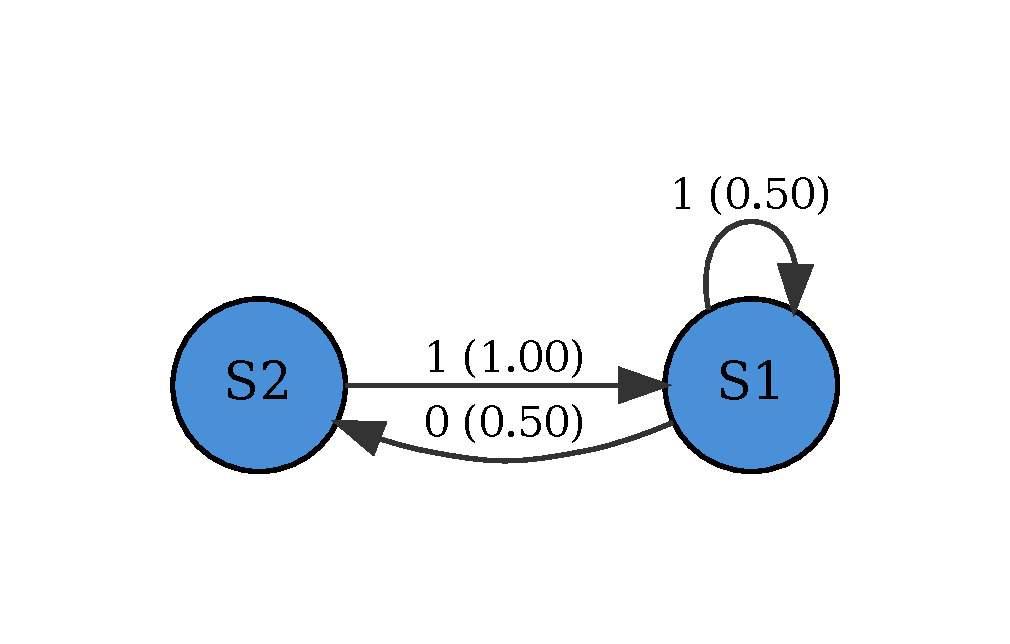
\includegraphics[width=\columnwidth]{figures/golden_mean_machine.pdf}
\end{emicfigure}

\subsection{Reading the Machine}
Look at the graph in Figure \ref{fig:gm_machine}.
\begin{itemize}
    \item \textbf{States}: There are two states. Let's call them $A$ and $B$.
    \item \textbf{Transitions}:
    \begin{itemize}
        \item From $A$, we can see '1' (loop back to $A$) or '0' (go to $B$).
        \item From $B$, we \textit{only} see '1' (and go back to $A$).
    \end{itemize}
\end{itemize}

Wait, does this match our rule?
\begin{itemize}
    \item State $A$ represents the condition "Last symbol was a 1". Since the last symbol was 1, we are free to emit 0 or 1 next.
    \item State $B$ represents the condition "Last symbol was a 0". Since the last symbol was 0, the rule says we \textit{must} emit a 1. So there is only one arrow leaving $B$.
\end{itemize}

The $\epsilon$-machine has automatically discovered the "No 00" rule just from the data! It identified that "histories ending in 0" have different predictive consequences than "histories ending in 1".


\section{Measures of Complexity}
\label{sec:measures}

Once we have the $\epsilon$-machine, we can calculate intrinsic properties of the process that go beyond simple statistics.

\subsection{Definitions}
We care about two fundamental quantities: structure and randomness.

\begin{description}
    \item[Statistical Complexity ($C_\mu$)] \hfill \\
    How much memory does the process need to store?
    It is defined as the Shannon entropy of the causal states themselves.
    \begin{equation}
        C_\mu = H[\mathcal{S}] = - \sum_{\sigma \in \mathcal{S}} \pi(\sigma) \log_2 \pi(\sigma)
    \end{equation}
    where $\pi(\sigma)$ is the probability of being in state $\sigma$.

    \item[Entropy Rate ($h_\mu$)] \hfill \\
    How random is the next symbol, given the past?
    It is the average uncertainty of the next symbol, averaged over the causal states.
    \begin{equation}
        h_\mu = H[X|\mathcal{S}] = \sum_{\sigma \in \mathcal{S}} \pi(\sigma) H[X|\sigma]
    \end{equation}
\end{description}

\begin{sidebar}{Intuition: Stored vs. Generated Information}
These two measures give us a complete picture of the process's information budget:
\begin{enumerate}
    \item $C_\mu$ is the information \textbf{stored} from the past. It represents \textit{Structure}.
    \item $h_\mu$ is the new information \textbf{generated} at each step. It represents \textit{Randomness}.
\end{enumerate}

\par\vspace{2mm}\hrule\vspace{2mm}

\textbf{Examples:}
\begin{itemize}
    \item \textbf{Clock}: High $C_\mu$ (many states to track), Zero $h_\mu$ (perfectly predictable).
    \item \textbf{Fair Coin}: Zero $C_\mu$ (no memory needed), High $h_\mu$ (maximum surprise).
\end{itemize}
\end{sidebar}

\subsection{Calculation}

Let's compute these values for our Golden Mean process ($p=0.5$).

\begin{sidebar}{Derivation for Golden Mean}
    \textbf{1. Statistical Complexity ($C_\mu$)}

    The stationary distribution over states is derived from the transition matrix. For the Golden Mean ($p=0.5$):
    \[ \pi(A) = 2/3, \quad \pi(B) = 1/3 \]
    The entropy of this distribution is:
    \begin{align*}
    C_\mu &= - \sum \pi(\sigma) \log_2 \pi(\sigma) \\
          &= - (2/3 \log_2 2/3 + 1/3 \log_2 1/3) \\
          &\approx 0.918 \text{ bits}
    \end{align*}

    \textbf{2. Entropy Rate ($h_\mu$)}

    This is the average uncertainty of the next symbol given the current state.
    \begin{itemize}
        \item State $A$ emits $0$ or $1$ with equal probability: $H[X|A] = 1$ bit.
        \item State $B$ always emits $1$: $H[X|B] = 0$ bits.
    \end{itemize}
    Weighted by state probability:
    \begin{align*}
    h_\mu &= \sum \pi(\sigma) H[X|\sigma] \\
          &= (2/3 \times 1) + (1/3 \times 0) \\
          &= 0.667 \text{ bits}
    \end{align*}
\end{sidebar}

\subsection{Comparison of Processes}
Different processes occupy different places on the complexity-entropy plane.

\begin{emictable}[label=tab:measures]{Measures for Common Processes}
\begin{tabular}{lp{3.5cm}ll}
\toprule
Process & Description & $C_\mu$ & $h_\mu$ \\
\midrule
\textbf{Fair Coin} & No memory, pure randomness. & 0.00 & 1.00 \\
\textbf{Period-2} & Alternating 0101... Needs 1 bit of memory. & 1.00 & 0.00 \\
\textbf{Golden Mean} & No '00'. A mix of structure and choice. & 0.92 & 0.67 \\
\bottomrule
\end{tabular}
\end{emictable}


\section{How Good is Our Prediction?}
\label{sec:theorems}

We have built machines that \textit{seem} to capture the structure of a process. We calculated their complexity and entropy. But how do we know if they are actually \textit{good} models?

Shalizi and Crutchfield (2001) give us two powerful guarantees---two "Fundamental Theorems" of Computational Mechanics.

\subsection{Theorem 1: Prescience (Accuracy)}

The first question is simple: \textbf{Does our model predict the future as well as the past allows?}

Imagine an Oracle who remembers the \textit{entire} infinite history of the universe ($\overleftarrow{X}$). We, on the other hand, only know the current causal state ($\mathcal{S}$).
Theorem 1 states that valid causal states are \textbf{prescient}:
\[ P(\vec{X} | \mathcal{S}) = P(\vec{X} | \overleftarrow{X}) \]
In English: \textit{Knowing the causal state is just as good as knowing the entire history.} You lose zero predictive power by compressing the history into a state.

\begin{intuition}
    \textbf{The Cost of Being Wrong: KL Divergence}\\
    To measure how wrong a model is, we use the \textbf{Kullback-Leibler (KL) Divergence}. Think of it as a "distance" between two probability distributions.

    If the true distribution of future symbols is $P$ and our model predicts $Q$, the KL divergence $D_{KL}(P || Q)$ tells us how many extra bits we need to correct our mistake.
    \begin{itemize}
        \item If $D_{KL} = 0$, our model is perfect.
        \item If $D_{KL} > 0$, our model is missing something.
    \end{itemize}
\end{intuition}

We can verify this theorem numerically. In \texttt{emic}, we can sweep through different complexity levels (by adjusting the significance level $\alpha$ of the statistical test) and measure the error.

\begin{emiclisting}[label=lst:optimality]{Checking Optimality}
\begin{lstlisting}[language=Python, basicstyle=\tiny\ttfamily, numbers=none]
# Does adding more states reduce error?
results = []
for alpha in [0.001, 0.01, 0.1, 0.5]:
    # Infer machine with decreasing strictness
    machine = cssr.infer(data, alpha)
    # Measure complexity (C_mu) and error (excess entropy)
    results.append((machine.c_mu, machine.kl_divergence))
\end{lstlisting}
\end{emiclisting}

In Figure \ref{fig:optimality}, we plot the prediction error (KL Divergence) against the number of states.

\begin{emicfigure}[label=fig:optimality]{The Optimality Curve}
    \centering
    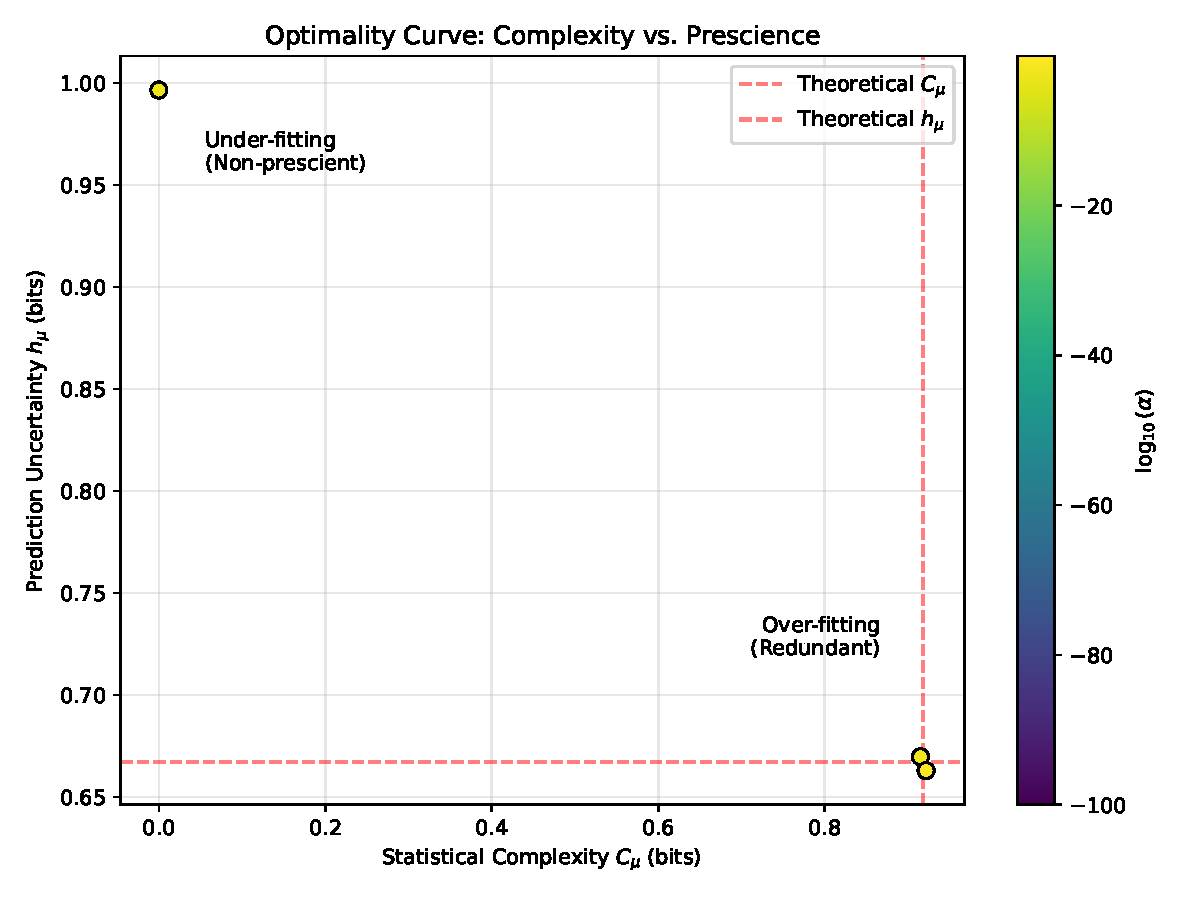
\includegraphics[width=\columnwidth]{figures/optimality_curve.pdf}

    The x-axis is complexity (number of states), the y-axis is prediction error ($D_{KL}$). The $\epsilon$-machine sits at the "elbow": minimal complexity for zero error.
\end{emicfigure}

Notice the curve. As we add more states (moving to the right), the error drops. But once we hit the "correct" number of states (the $\epsilon$-machine), the error hits zero. Adding more states after that point doesn't help---it just wastes memory.

\subsection{Theorem 2: Minimality (Efficiency)}

The second question is about efficiency: \textbf{Is this the smallest possible correct model?}

You could predict the future perfectly by simply memorizing every sequence of length 1000. That would be "prescient" (zero error), but it would be huge ($2^{1000}$ states!).

Theorem 2 states that among all prescient models, the $\epsilon$-machine is the \textbf{minimal} one. It has the smallest possible statistical complexity ($C_\mu$).
\[ C_\mu(\epsilon\text{-machine}) \leq C_\mu(\text{any other prescient model}) \]

This confirms that the $\epsilon$-machine is the \textbf{unique, simplest, optimal predictor} of a process.


\section{From Rules to Chaos}
\label{sec:chaos}

We have seen simple processes like the Golden Mean, which require only a few bits of memory. But what happens when we look at complex physical systems?

One of the most surprising discoveries of the 20th century was \textbf{Chaos}: simple deterministic rules can produce behavior that looks completely random. Computational Mechanics gives us a toolkit to "measure" this chaos. It allows us to ask: \textit{Is this randomness "simple" (like a coin flip) or "complex" (requiring memory)?}

\subsection{The Logistic Map}
Consider a simple model of population growth, the Logistic Map:
\[ x_{n+1} = r x_n (1 - x_n) \]
where $x_n$ is the population at year $n$, and $r$ is the growth rate.

As we increase $r$, the behavior undergoes a dramatic transformation:
\begin{itemize}
    \item \textbf{Order ($r < 3$)}: The population settles to a single stable value.
    \item \textbf{Periodicity ($r \approx 3.5$)}: The population bounces between 2, 4, 8... values.
    \item \textbf{Chaos ($r \approx 4.0$)}: The population jumps wildly and unpredictably.
\end{itemize}

\subsection{The Structure of Chaos}
We can convert this numerical data into symbols: '1' if the population is high ($x > 0.5$), '0' if low. Then, we use \texttt{emic} to infer the $\epsilon$-machine at each value of $r$.

\begin{emiclisting}[label=lst:chaos]{Scanning for Chaos}
\begin{lstlisting}[language=Python, basicstyle=\tiny\ttfamily, numbers=none]
# Scan the parameter r
for r in np.linspace(3.5, 4.0, 100):
   data = logistic_map(r, size=10000)
   machine = cssr.infer(data)
   # How much memory does the process need?
   complexity = machine.statistical_complexity()
\end{lstlisting}
\end{emiclisting}

The results, shown in Figure \ref{fig:logistic}, reveal the hidden architecture of chaos.

\begin{emicfigure}[float*=t, label=fig:logistic]{The Architecture of Chaos}
    \centering
    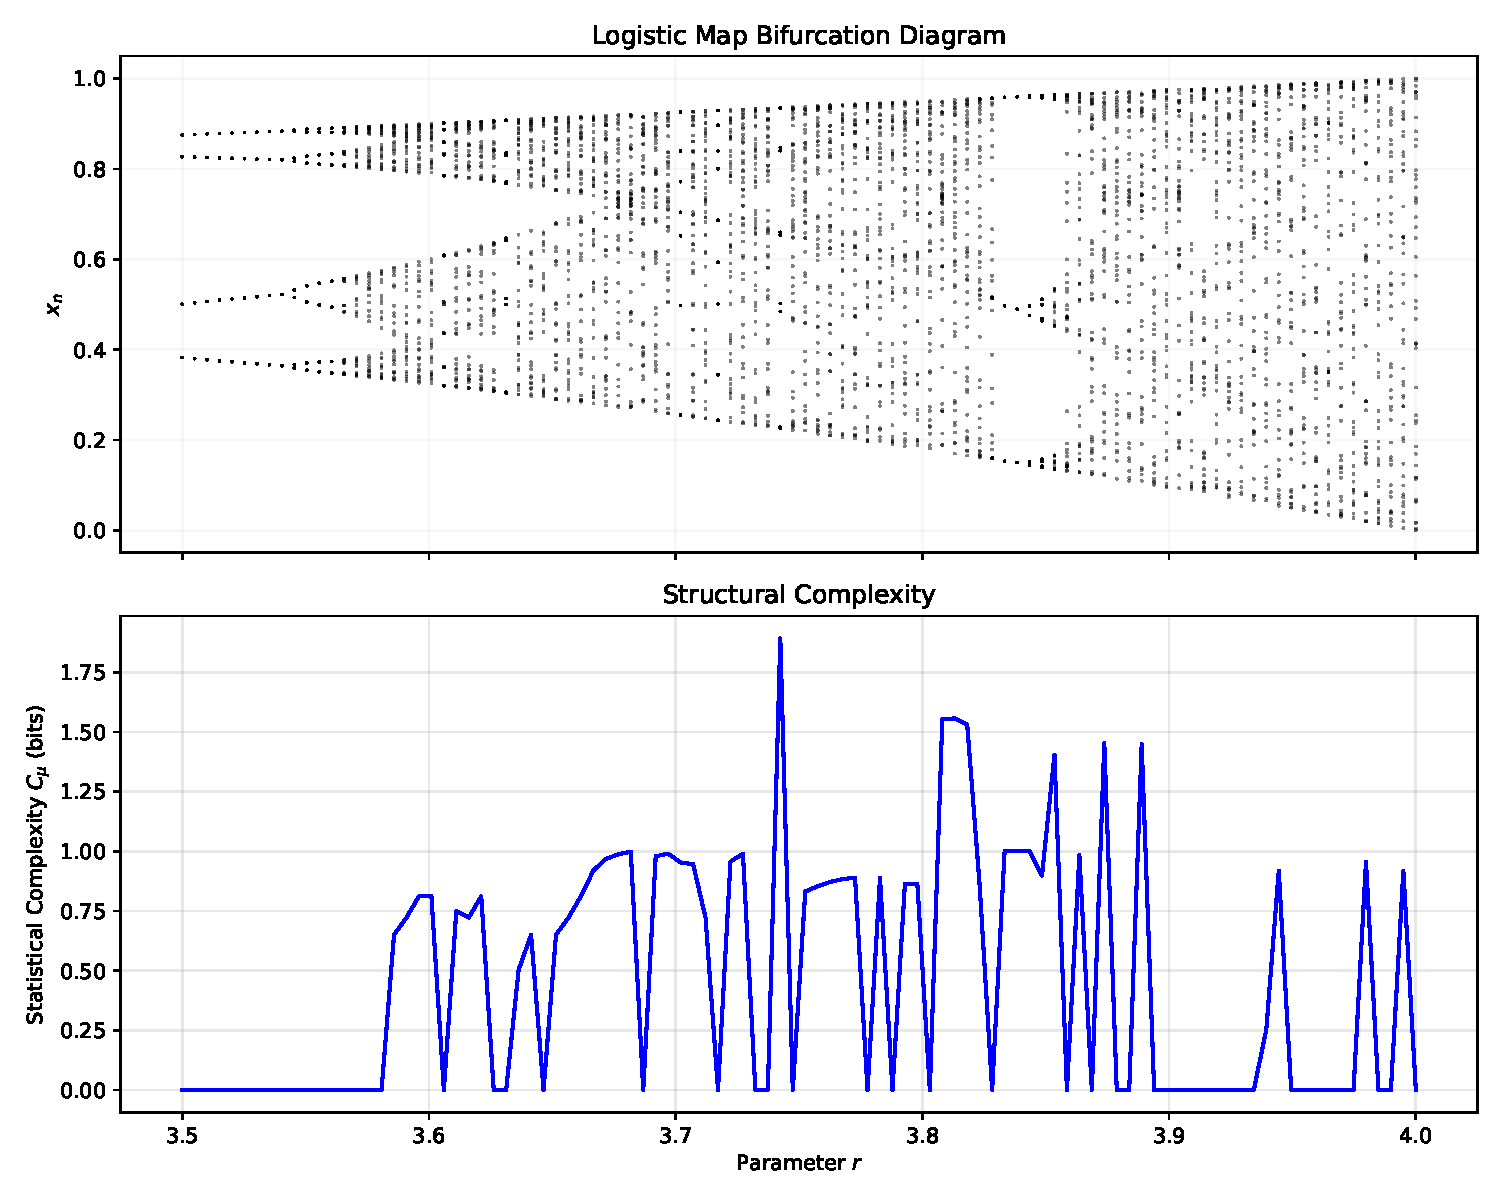
\includegraphics[width=\textwidth]{figures/logistic_complexity.pdf}

    Top: The bifurcation diagram (values of $x$). Bottom: Structural complexity ($C_\mu$).
\end{emicfigure}

\begin{intuition}
    \textbf{The Edge of Chaos}\\
    Look at the blue curve (Statistical Complexity).
    \begin{itemize}
        \item In the \textbf{Ordered} regime, complexity is low. It's easy to predict a fixed point.
        \item In the \textbf{Chaotic} regime (far right), complexity is \textit{also} low! If a system is completely random, you don't need memory to predict it---you just guess.
        \item The peaks occur at the \textbf{transition}, the "Edge of Chaos".
    \end{itemize}
    This tells us something profound: \textbf{Structure lives in the balance between order and randomness.}
\end{intuition}


\section{Conclusion: The Physics of Information}
\label{sec:conclusion}

We began this guide with a simple question: \textit{How do we find pattern in randomness?}

Through the lens of Computational Mechanics, we have seen that "pattern" is not just a vague visual concept. It is a physical quantity that can be measured, derived, and understood.

\begin{enumerate}
    \item \textbf{History matters:} We saw that the past influences the future, but not all pasts are created equal.
    \item \textbf{States are summarized histories:} By grouping equivalent histories into \textbf{Causal States}, we found the minimal necessary information to predict the future.
    \item \textbf{Machines can be inferred:} using algorithms like CSSR, we can reconstruct the $\epsilon$-machine purely from data, as we did with the Golden Mean.
    \item \textbf{Complexity is physically meaningful:} We discovered that structure ($C_\mu$) peaks not in total order or total chaos, but at the phase transitions between them.
\end{enumerate}

This framework transforms "Information" from a static quantity (bits in a hard drive) into a dynamical one (bits required to predict). Whether you are studying the string of DNA code, the fluctuations of a stock market, or the firing of neurons, the $\epsilon$-machine gives you the intrinsic architecture of the process.

We invite you to use the \texttt{emic} library to explore your own data. The tools we used here---generating data, inferring states, calculating complexity---are available for you to discover the hidden structure in your own world.

\subsection*{Further Reading}
\begin{itemize}
    \item Shalizi, C. R., \& Crutchfield, J. P. (2001). \textit{Computational mechanics: Pattern and prediction, structure and simplicity}.
    \item Crutchfield, J. P. (2012). \textit{Between order and chaos}. Nature Physics.
\end{itemize}


\bibliographystyle{plain}
\bibliography{references}

\end{document}
